% Copyright 2009 by Tomasz Mazur
% This file may be distributed and/or modified in all ways.

%\documentclass[xcolor=pdftex,t,11pt,handout]{beamer}
\documentclass[xcolor=pdftex,t,11pt]{beamer}

%%%%%%%%%%%%%%%%%%%%%%%%%%%%%%%%%%
%       SET OPTIONS BELOW        %
%%%%%%%%%%%%%%%%%%%%%%%%%%%%%%%%%%
\usepackage[icelandic, english]{babel}
\usepackage{t1enc} 
\usepackage{textcomp}
\usepackage[
% Toggle showing page counter
pagecounter=true,
%
% String to be used between the current page and the
% total page count, e.g. of, /, from, etc.
pageofpages=of,
%
% Defines the shape of bullet points. Available options: circle, square
bullet=circle,
%
% Show a line below the frame title. 
titleline=true,
%
% Set the style of the title page (true for fancy, false for standard)
alternativetitlepage=true,
%
% Institution logo for fancy title page.
titlepagelogo=presentation/beamer/hilogo,
ordinarypageslogo=presentation/beamer/hilogo,
]{presentation/beamer/beamerthemeBerkeley} 

% Select color theme. Available options are:
% mininmal, greenandblue, blue, red
\usepackage{presentation/beamer/beamercolorthemehi}

%Select different font themes.Available options are:
% default, serif, structurebold, structureitalicserif, structuresmallcapsserif
\usefonttheme{structurebold}

\setbeamercovered{transparent}

\newcommand{\bi}{\begin{enumerate}[label={{$\star$}}]\item }
\newcommand{\ei}{\end{enumerate}}

\usepackage{ifthen}
\usepackage{float}
\usepackage{morefloats}

\usepackage{footnote}
\usepackage[bottom,perpage,symbol*]{footmisc}

\newcommand{\tcr}[1]{{\color{red} #1}}
\newcommand{\tcb}[1]{{\color{blue} #1}}
\newcommand{\tcg}[1]{{\color{green} #1}}
\newcommand{\Alice}{Alice}
\newcommand{\fullnameAlice}{Adaptive Learning Intelligent Composite rulEs}
 % put your own shorthand declarations here
\usepackage{longtable}
\usepackage{tabularx}
\usepackage{multirow}
\usepackage{rotating}
\newcommand{\rot}[1]{\begin{sideways}#1\end{sideways}}


\setlist[description]{leftmargin=1cm,labelindent=1cm}
\usepackage[retainorgcmds]{packages/IEEEtrantools}
\usepackage{nicefrac}
\usepackage{booktabs} % \toprule \midrule \bottomrule

\usepackage{comment}
\usepackage[splitrule,bottom,perpage,symbol*]{packages/footmisc}
\setfnsymbol{wiley} % wiley: ∗, ∗∗, †, ‡, §, ¶, ||.
\renewcommand{\mpfootnoterule}{}
\let\splitfootnoterule\footnoterule
\renewcommand{\thempfootnote}{\fnsymbol{mpfootnote}}

\usepackage{aliascnt}
\usepackage[capitalise,nameinlink]{cleveref} % must come last! 
% provide singular and plural names of the categories "paper"
\crefname{paper}{Paper}{Papers}
\Crefname{paper}{Paper}{Papers}
\crefname{ineq}{Ineq.}{Ineqs.}
\Crefname{ineq}{Inequality}{Inequalities}
\creflabelformat{ineq}{~\upshape(#2#1#3)}

\usepackage{soul} % strikeout text \st{text}
%\setstcolor{gray}

\usepackage{algorithm}
\usepackage{algpseudocode}
\makeatletter
\def\BState{\State\hskip-\ALG@thistlm}
\makeatother
\algnewcommand\algorithmicto{~\textbf{to}~}
\algnewcommand\algorithmicand{~\textbf{and}~}
\algrenewtext{For}[3]%
{\algorithmicfor\ $#1 \gets #2 \text{\algorithmicto} #3$~\algorithmicdo}

\newcommand{\ntodo}[2][]{\todo[#1]{\thesection{}. #2}}
\newcommand{\todoFind}[1]{\ntodo[color=red]{#1}}
\newcommand{\todoExtend}[1]{\ntodo[color=blue]{#1}}
\newcommand{\todoPapers}[1]{\ntodo[color=green]{#1}}
\newcommand{\todoWrite}[1]{\ntodo[inline,color=yellow]{#1}}

\usepackage{packages/forest} % for figures/orlib-methods
\tikzstyle{arrow} = [->,>={latex}, draw=black]

% ------------------------------------------------------- for alice.tex
\usepackage{etoolbox}
\newcommand\chquote[3][]{%
    \ifstrempty{#1}{%
        \emph{#3} 
    }{%
    #1: \emph{\st{#3}} 
}%
\hfill \textbf{#2}\\\\
}
 % put your own shorthand declarations here

\graphicspath{{presentation/},{figures/}}
\DeclareGraphicsExtensions{.eps,.png}
%%%%%%%%%%%%%%%%%%%%%%%%%%%%%%%%%%
%       PRESENTATION INFO        %
%%%%%%%%%%%%%%%%%%%%%%%%%%%%%%%%%%
\author[Helga]{Helga Ingimundard\'{o}ttir}
\title{\Alice}
\subtitle{\fullnameAlice}
\institute{University of Iceland}	
\date{June 30, 2016}

\newcommand<>{\tikzMe}[1]{% previously: \def\tikzMe<#1>#2{…
    \tikz[baseline]\node[BeamerAlert=#2,anchor=base] {#1};
}

\begin{document}

%%%%%%%%%%%%%%%%%%%%%%%%%%%%%%%%%%
%       SLIDE DEFINITIONS        %
%%%%%%%%%%%%%%%%%%%%%%%%%%%%%%%%%%

\begin{frame}
	\titlepage
\end{frame}

\section{Introduction}
\frame{
\frametitle{Introduction}
Motivation
\bi The general goal is to train optimisation algorithms, for an 
arbitrary problem domain, using data\ei
Contribution
\bi The main contribution of this thesis is towards a better understanding of 
how this training data should be constructed\ei 
}
\frame[label=alice]{
    \frametitle{Framework for Algorithm Learning}
    \setbeamercovered{invisible}
\begin{figure}[t]\centering
\tikzset{
    block/.style = {draw, fill=gray!10, rectangle, text width=7em, 
        align=center,font=\bfseries\sffamily},
    txt/.style = {font=\small\sffamily,text width=9em,align=center,midway},
    ltxt/.style = {txt,left,align=right},
    rtxt/.style = {txt,right,align=left},
    rice/.style = {beameralert=1},    
    invisible/.style={opacity=0,text opacity=0},
    visible on/.style={alt=#1{}{invisible}},
    alt/.code args={<#1>#2#3}{%
        \alt<#1>{\pgfkeysalso{#2}}{\pgfkeysalso{#3}} 
    },
    beameralert/.style={alt=<#1>{fill=red!50}{},anchor=base},
}
\vspace{-12pt}
\resizebox{\columnwidth}{!}{%
% The block diagram code is probably more verbose than necessary
\begin{tikzpicture}[auto, node distance=2.3cm]%,>=latex']
\node [block, rice, beameralert=2, beameralert=9] (P) {Problem space 
$\vec{z}\in\mathcal{P}$};
\node [block, beameralert=3, beameralert=10, below of=P] (I) {Subspace of 
instances \mbox{$\vec{x}\in \mathcal{P}' \subset \mathcal{P}$}};
\node [block, rice, beameralert=4, beameralert=11, below of=I] (Phi) {Feature 
space $\vphi(\vec{x})\in\Phi\subset\mathcal{F}$};
\node [block, beameralert=7, beameralert=16, right of=P, xshift=3.4cm] (F) 
{Footprints in instance space};
\node [block, rice, beameralert=6, beameralert=15, right of=I, xshift=3.4cm] 
(Y) {Performance space $y\in\mathcal{Y}$};
\node [block, rice, beameralert=5, beameralert=14, right of=Phi, xshift=3.4cm] 
(A) {Algorithm space $a\in\mathcal{A}$};

\draw [arrow] (P) -- node[ltxt] {instance selection} (I);
\draw [arrow] (I) -- node[ltxt] {feature selection $\vphi$} (Phi);
\draw<1-7>[arrow] (Phi) -- (A);
\draw [arrow] (A) -- node[rtxt] {$\Upsilon(a,\vphi(\vec{x}))$ apply alg. $a$ to 
    instance $\vec{x}$} (Y);
\draw [arrow] (Y) -- node[rtxt] {define algorithm footprint 
    $f(y(a,\vec{x}))$} (F);
\draw [arrow] (F) -- node[txt] {infer algorithm performance on all 
    $\vec{z}\in\mathcal{P}$} (P);
\visible<8->{
\node [block, beameralert=12, below of=Phi] (Psi) {Preference 
set $\Psi \subset \Phi$};
\node [block, beameralert=13, right of=Psi, xshift=3.4cm] 
(PREF) {Preference learning};
\draw [arrow] (Phi) -- node[ltxt] {sample preference pairs} (Psi);
\draw [arrow] (Psi) -- (PREF);
\draw [arrow] (PREF) -- node[rtxt] {train algorithm $a$} (A);
}
\visible<8->{
    \draw [arrow,dotted] (F) -- node[txt,sloped,above] {feedback} (Psi);
}
\end{tikzpicture}}
\end{figure}
}

\section{Problem space}\againframe<1>{alice}

\section{Subspace of instances}\againframe<2>{alice}

\section{Feature Space}\againframe<11|handout:0>{alice}
\frame{\frametitle{Feature Space}\framesubtitle{for \jsp}
    \begin{table}[t!] \centering
    \vspace{-14pt}
    \resizebox{\textheight}{!}
    {\scriptsize 
    \renewcommand{\arraystretch}{0.6}
    \begin{tabular}{ccl}
        \toprule
        %& $\vphi$ & Feature description \\  \midrule
        \multirow{10}{*}{\rot{\textbf{job}}}
        & \alert<2>{$\phiproc$} & \alert<2>{job processing time} \\
        & $\phistartTime$ & job start-time \\
        & $\phiendTime$ & job end-time \\
        & $\phiarrivalTime$ & job arrival time \\ 
        & $\phiwait$ & time job had to wait \\ 
        & $\phijobTotProcTime$ & total processing time for job \\
        & \alert<3>{$\phijobWrm$} & \alert<3>{total work remaining for job} \\
        & $\phijobOps$ & number of assigned operations for job \\ 
        \midrule
        \multirow{10}{*}{\rot{\textbf{machine}}}
        & $\phimacFree$ & when machine is next free \\
        & $\phimacTotProcTime$ & total processing time for machine \\
        & $\phimacWrm$ & total work remaining for machine \\
        & $\phimacOps$ & number of assigned operations for machine \\
        & $\phireducedSlack$ & change in idle time by assignment \\
        & $\phimacSlack$ & total idle time for machine \\
        & $\phiallSlack$ & total idle time for all machines \\
        & $\phimakespan$ & current makespan \\
        \midrule
        \multirow{12}{*}{\rot{\textbf{final makespan}}}
        & $\phiSPT$ & final makespan using SPT \\
        & $\phiLPT$ & final makespan using LPT \\
        & $\phiLWR$ & final makespan using LWR \\
        & $\phiMWR$ & final makespan using MWR \\
        & $\phiRND$ & final makespans using 100 random rollouts \\ 
        & $\phiRNDmean$ & mean for $\phiRND$ \\ 
        & $\phiRNDstd$ & standard deviation for $\phiRND$ \\
        & $\phiRNDmin$ & minimum value for $\phiRND$\\ 
        & $\phiRNDmax$ & maximum value for $\phiRND$\\ 
        \bottomrule
    \end{tabular}
    }
    \end{table}\pause\pause
}

\frame{\frametitle{Trajectory Strategies for \PhiSet{}}\framesubtitle{}
    Following the \alert<1-7>{policy}
    \bi \alert<1>{(\PhiSet{\OPT})} expert $\pi_\star$.
    \pause \item \alert<2>{(\PhiSet{\SPT})} shortest processing time (SPT).
    \pause \item \alert<3>{(\PhiSet{\LPT})} longest processing time (LPT).
    \pause \item \alert<4>{(\PhiSet{\LWR})} least work remaining (LWR).
    \pause \item \alert<5>{(\PhiSet{\MWR})} most work remaining (MWR).
    \pause \item \alert<6>{(\PhiSet{\RND})} random policy (RND).
    \pause \item \alert<7>{(\PhiSet{\minRho})} the policy obtained by 
    optimising with CMA-ES. 
    \pause \item \alert<8>{(\PhiSet{\ALL})} union of all of the above\ei
}

\frame[label=featsize]{
    \frametitle{Sampled Size of $\abs{\Phi(k)}$}
    \framesubtitle{$6\times5, N_{train}=500$}
    \begin{center}    
        \includegraphics[width=\columnwidth]{presentation/{trdat.size.6x5}.pdf}
    \end{center}    
}

\section{Algorithm space}\againframe<4>{alice}
\section{Performance space}\againframe<15|handout:0>{alice}
\frame{\frametitle{Performance measure}
     Performance of policy $\pi$ compared with its optimal makespan, found 
     using an expert policy, $\pi_{\star}$, is the following loss function: 
     $$\rho=\frac{C_{\max}^{\pi}-C_{\max}^{\pi_\star}}{C_{\max}^{\pi_\star}}\cdot
      100\%$$
    The goal is to minimise this discrepancy between \alert{predicted} value 
    and \alert{true} outcome. 
 }
\section{Footprints in instance space}\againframe<6>{alice}
\frame{\frametitle{\Namerho}
\includegraphics[width=\columnwidth]{presentation/{boxplot.6x5.SDRs}.pdf}   
}
\section{Preference set}\againframe<7>{alice}
\frame{\frametitle{Generating training data}
    \Alice\ framework for creating \dr s
    \bi \alert{Linear classification} to identify good dispatches, 
    from worse ones. 
    \pause \item Generate feature set, $\Phi\subset\mathcal{F}$, both from 
    \bi \alert{optimal} solutions, $\vphi^o$ 
    \item \alert{suboptimal} solutions, $\vphi^s$\ei 
    by exploring various \alert{trajectories} within the feature-space 
    (where $\vphi^o,\vphi^s\in\mathcal{F}$).
    \pause \item Sample $\Phi$ to create training set $\Psi$ with rank 
    pairs:
    \bi \alert{optimal} decision, $(\vec{z}^o,y_o)=(\vphi^o-\vphi^s,+1)$ 
    \item \alert{suboptimal} decision, $(\vec{z}^s,y_s)=(\vphi^s-\vphi^o,-1)$\ei
    using different \alert{ranking} schemes 
    (where $\vec{z}^o,\vec{z}^s\in\Psi$) 
    \pause \item Sample $\Psi$ using \alert{stepwise bias} for time independent 
    policy\ei
}

\frame{\frametitle{Ranking schemes for \PsiSet{}}
    Sampling rankings of available jobs where where $r_1>r_2>\cdots>r_{n'}$ 
    $(n'\leq n)$ with respect to
    \pause\bi[\PsiSet{b}] all opt rankings $r_1$ vs. all possible subopt 
    rankings $r_i$, $i\in\{2,...,n'\}$
    \pause\item[\PsiSet{f}] full subsequent rankings, i.e., all combinations of 
    $r_i$ and $r_{i+1}$ for all $i\in\{1,...,n'\}$. 
    \pause\item[\PsiSet{p}] partial subsequent rankings, similar to \PsiSet{f}
    except if there are more than one operation with the same rank, only one 
    is needed to be compared to subsequent rank     
    (\PsiSet{p}$\subset$\PsiSet{f}).
    \pause\item[\PsiSet{a}] union of all of the above\ei
}

\frame{\frametitle{Sampled size of $\abs{\Psi}$ 
        ($6\times5, N_{train}=500)$}
    \vspace{-12pt}
    \begin{center}   
        \includegraphics[height=.95\textheight]{figures/{prefdat.p.size.6x5}.pdf}
    \end{center}    
}

\frame{\frametitle{Stepwise bias for sampling \PsiSet{}}
    Sampling stepwise bias for preference pairs
    \pause\bi \textbf{(equal)} equal probability. 
    \pause\item \textbf{(opt)} inverse optimality for random dispatches
    -- $1-\xi_{\RND}^{\star}$.
    \pause\item \textbf{(bcs)} best case scenario for mean $\rho$ 
    -- $\zeta^{\star}_{\min}$.
    \pause\item \textbf{(wcs)} worst case scenario for mean $\rho$ 
    -- $\zeta^{\star}_{\max}$.
    \pause\item \textbf{(featsize)} inversely proportional to 
    $\abs{\Phi^{\OPT}}$
    \pause\item \textbf{(prefsize)} inversely proportional to 
    $\abs{\Psi^{\OPT}_p}$
    \pause\item \textbf{(dbl1st)} \label{bias:dbl1st} twice as much weight on 
    the first half of the dispatches.
    \pause\item \textbf{(dbl2nd)} twice as much weight on the second half of 
    the dispatches\ei
}

\frame{\frametitle{Stepwise bias strategies}
    \includegraphics[width=\columnwidth]{figures/{bias.CDR.10x10}.pdf}
}

\section{Preference learning}\againframe<8>{alice}
\frame{\frametitle{Ordinal Regression}
    Preference learning
    \bi Mapping of points to ranks: $ \{h(\cdot) : \Phi \mapsto Y\}$ where 
    $$\vphi_o \succ \vphi_s \quad \iff \quad h(\vphi_o) > h(\vphi_s)$$
    \item The preference is defined by a linear function:
    $$ h(\vphi) = \sum_{i=1}^d w_i \vphi $$
    based on $d$ features -- optimised w.r.t. $\vec{w}$\ei	
}
\frame{\frametitle{Learning methods}
    Passive imitation learning
        \bi Prediction with expert advice, $\pi_\star$ -- Gurobi\ei
    \pause 
    Active imitation learning
        \bi Follow the perturbed leader (OPT$\epsilon$)
        \pause\item Dataset Aggregation (DAgger)
        $$ \pi_i = \beta_i \pi_\star + (1-\beta_i)\hat{\pi}_{i-1}$$
        where $\hat{\pi}_{i-1}$ is the previous learned model, \pause and 
        $\hat{\pi}_i$ learns on
        $$ \Phi^{\text{DA}i} = \bigcup_{i'=0}^i \Phi^{\text{IL}i'}$$
        aggregated dataset of all previous iterations\ei   
}
\frame{\frametitle{DAgger}
\begin{algorithmic}[1]
\Require $T\geq1$
\Procedure{DAgger}{$\pi_\star,\Phi^{\IL{0}},T$}
    \State $\hat{\pi}_0 \gets$ \Call{Train}{$\Phi^{\IL{0}}$}
        \Comment{initial model, iff $\Phi^{\IL{0}}=\Phi^{\OPT}$}
\pause 
    \For{i}{1}{T} \Comment{at each imitation learning iteration}
\pause 
        \State Let $\pi_i = \beta_i\pi_\star + (1-\beta_i)\hat{\pi}_{i-1}$
\pause 
        \State Sample a $K$-solution using $\pi_i$
            \Comment{\Call{IL}{$i,\hat{\pi}_{i-1},\pi_\star$}}
\pause      
        \State $\Phi^{\IL{i}} = \{(s,\pi_\star(s))\}$ 
            \Comment{visited by $\pi_i$ and actions by $\pi_\star$}
\pause           
        \State $\Phi^{\DA{i}} \gets \Phi^{\DA{i-1}} \cup \Phi^{\IL{i}}$ 
            \Comment{aggregate datasets}
\pause
        \State $\hat{\pi}_{i+1} \gets$ \Call{Train}{$\Phi^{\DA{i}}$}
            \Comment{preference model}
    \EndFor
\pause
    \State \Return best $\hat{\pi}_i$ on validation \Comment{best preference 
    model}
\EndProcedure
\end{algorithmic}
    
}
\frame{\frametitle{\Namerho}
    \includegraphics[width=\columnwidth]{figures/{j.rnd}/{boxplot.summary.10x10}.pdf}
}
\section{Conclusions}\againframe<9>{alice}
\frame{\frametitle{Using \fullnameAlice\ framework I}
The thesis introduced a framework for learning (\alert<1>{linear}) \cdr\ -- 
using \alert<1>{\jsp} as a case-study -- with the following guidelines
\pause        
    \bi For a given problem domain, use a suitable problem \alert<2>{generator} 
    to \alert<2>{train} and \alert<2>{test} on.
\pause 
    \item Define \alert<3>{features} to grasp the essence of visited 
    \alert<3>{$k$-solutions}
\pause
\item \alert<4->{Success} is highly dependent on the preference pairs 
introduced to the system: 
\pause
    \bi \PsiSet{p} \alert<5>{reduces} the preference set without loss of 
    performance. 
\pause
    \item \alert<6>{Stepwise bias} is needed to balance time dependent 
    \PsiSet{p} in order to create \alert<6>{time independent} models. \ei
\pause 
    It is \alert<7>{non intuitive} how to go about \alert<7>{collecting} 
    training data\ei
}
\frame{\frametitle{Using \fullnameAlice\ framework II}
Continued from prev. slide
    \bi Learning \alert<1>{optimal} trajectories predominant in literature. 
    Study showed \PhiSet{\OPT} can result in \alert<1>{insufficient} knowledge.
\pause 
    \item Following \alert<2>{sub-optimal} deterministic policies, yet 
    labelling with an optimal solver, \alert<2>{improves} the guiding 
    policy.
\pause 
    \item In \alert<3>{sequential} decision making, all future observations are 
    dependent on \alert<3>{previous} operations.
\pause
    Active update procedure using \alert<4>{DAgger} ensures sample states the 
    \alert<4>{learned model is likely to encounter} is integrated to 
    \PsiSet[\DA{i}]{p}.
\pause
    \item Instead of reusing same problem instances, extend the training set 
    with \alert<5>{new} instances for \alert<5>{quicker convergence} of 
    DAgger\ei    
}
\frame{\frametitle{Future work}
    Main conclusions
    \bi \ei        
}



% uppskrift of how-to-make-an-algorithm

\frame{
\frametitle{Thank you for your attention}
\begin{columns}[T]
    \begin{column}{0.5\columnwidth} 
        \vspace{36pt}
        \begin{center}
            Helga Ingimundard\'{o}ttir\\
            \url{hei2@hi.is}
        \end{center}
        \vspace{36pt}
        Supplementary material
        \bi \href{https://tgax89.rhi.hi.is:3838/alice}{Shiny application}
            \item \href{https://github.com/ALICE-InRu/Cheshire}{Github} 
        \ei
    \end{column}
    \begin{column}{0.5\columnwidth}
        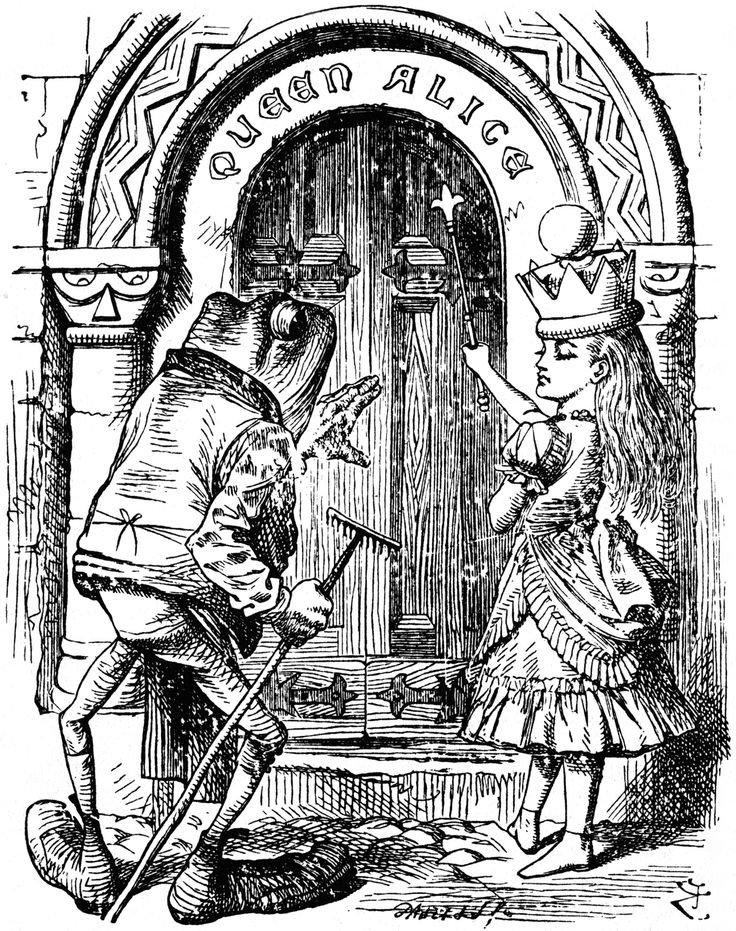
\includegraphics[width=\columnwidth]{tenniel/queen-alice.jpg}
    \end{column}    
\end{columns}
}
\end{document}